\section{Mesoscale operational oceanography}
\label{sec:operational_oceanography}
Tide prediction has effectively been in routine operations for several decades.
More recently, mesoscale ocean prediction moved into operations across the early 2000s in a manner that lagged and imitated the path of \NWP \citep{Harper:2008ub}. And like modern weather forecasting, operational oceanography is similarly a big science enterprise \citep{Petersen:2012tr} in the sense that it fundamentally relies on the coordination of large organisations, global networks and capital. 
The size and nature of this type of prediction stands in stark contrast to the ``small'' well-established practices of conventional tide prediction introduced in section \ref{sec:tidesOverview}.
The international Global Ocean Data Assimilation Experiment \GODAE{} serves as a historical reference point for how mesoscale prediction came into operational agencies like the Bureau:
``\textit{the central idea of \GODAE{} - to demonstrate the feasibility and utility of real-time, global ocean forecasting - was based on the experiences of the meteorological community in \dots{} FGGE}'' \citep{Bell:2009uv}.
From this original feasibility demonstration, the enterprise of mesoscale ocean forecasting has continued to mature across many national weather agencies; and the Australian case is documented by \cite{10.1080/1755876x.2019.1685834} in reviewing over 15 years of operational services.


In contrast to conventional tide prediction, sea level of itself is not the target of mesoscale forecasting; let alone coastal sea level.   But sea surface elevation is an important state variable for which forecasts are produced.  What these forecasts represent is not self-evident. And the manner in which sea level and tides are handled in systems like \BL{} is worthy of exposition in order to underpin the subsequent chapters describing methods for combining and evaluating sea level derived from these operational forecasts. 
  
%-----------------%
\subsection{Ocean general circulation models}
Ocean General Circulation Models (\OGCM{}s) are now a key component in oceanographic forecasting, but are only rendered operationally useful by the use of a global observation network and data assimilation to routinely maintain alignment with reality.
How this representation of reality relates to coastal sea level is however not self-evident.



An \OGCM{} simulates the physical ocean state via time step integrating a mixed boundary-condition/initial-condition problem.
In contrast to the tidal LTI conception of the ocean described in section \ref{sec:LTI}, an \OGCM{} conceives the global ocean as a turbulent continuum fluid; and the time and length scales of this turbulence effectively have no lower bound. The simulation thus needs to represent information cascades between turbulent scales as well as account for unresolved processes with sub-grid scale (SGS) parameterisations.
The distinction between resolved and unresolved scales is paramount.  ``Sensitive dependence on initial conditions in this turbulent flow \dots{} severely limits predictive capabilities [and] motivates a formulation of averaged or mean field fluid equations'' \citep[Sec 2.5]{Griffies:2004vs}.
Furthermore, this raises broad questions of how to interpret the output of a numerical ocean simulation.
Griffies perceives an \OGCM{} as representing the averaged motion of an infinite ensemble of hypothetical oceans; the imagined spread being proportional to the scales of SGS parameterisation.
Alternatively, \citet{Stevens:2001kb} casts \OGCM{}s into the class of geophysical ``pseudofluid'' simulations. Of which he notes comparisons with observational data are prone to interpretational nuance and are ``too often ad hoc, uncritical, and/or irrelevant''\citep[pp 286]{Stevens:2001kb}. 
Figure \ref{fig:ogcmScales} illustrates very schematically the place of \OGCM{} variants in the context of turbulence simulations.   The exclusion or explicit representation of tidal dynamics are shown as changes in SGS complexity; these are discussed further below.
%----------------------------------
\begin{figure}[h]\centering
  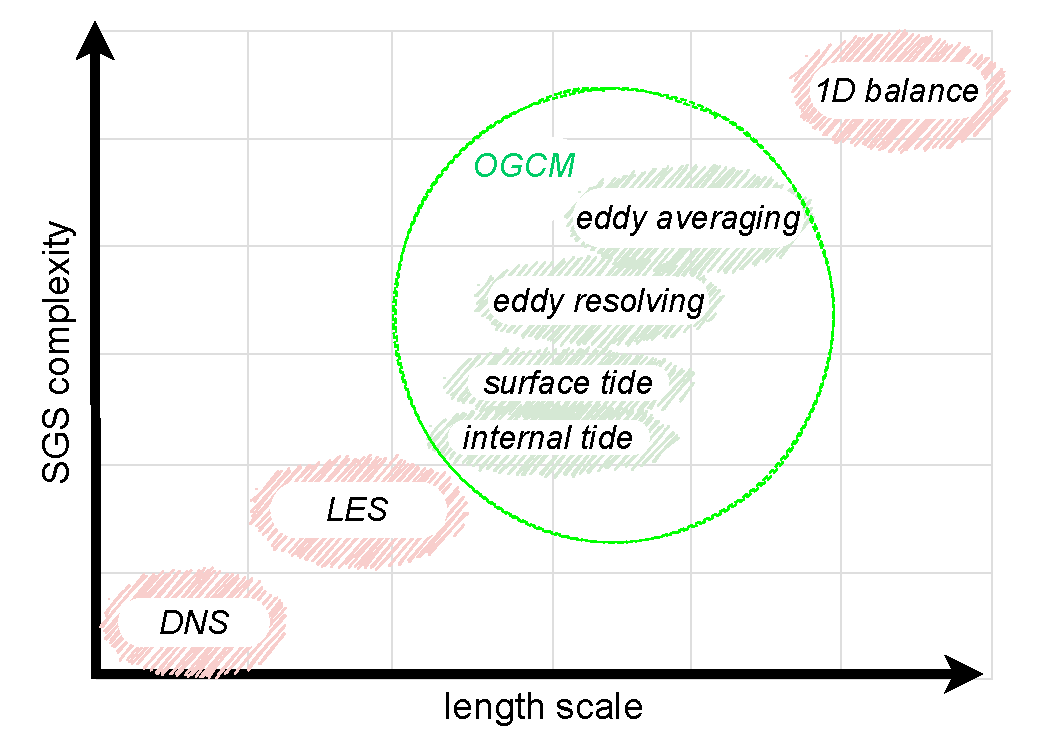
\includegraphics[width=\figwidthBig]{figures/diagrams/ogcm_scales.pdf}
  \caption{Schematic illustration of place of \OGCM{}s in terms of the sub-grid-scale (SGS) parameterisation of the broad scale range of a turbulent ocean.  For reference, methods from turbulence studies are included: Direct Numerical Simulation and Large Eddy Simulation. Following \citep[fig 5.2]{Petersen:2012tr} and \citep{Stevens:2001kb}.  Explicit tides in an OGCM represent a reduction of parameterisation without a large change in spatial scale resolution.}
  \label{fig:ogcmScales}
\end{figure}
%----------------------------------
Common to `big science' simulation practice more generally \citep{Petersen:2012tr} any real \OGCM{}, including \BL{}, embodies a significant accumulation of human effort in the very many lines of computer code.  In contrast to typical tidal analysis tools, the software behind a mesoscale ocean forecast is effectively too much for any one person to understand in detail.
%-----------------%
\subsection{Data assimilation and sea level observation}
Data assimilation is the model-data-fusion framework by which the initial conditions for each \OCGM{} forecast are determined.
This processing step can be usefully viewed from a Bayesian perspective in which ``the system implements an optimality criterion which defines how to best combine dynamics and observations, given an hypothesized error model for both.'' \citep{10.1007/978-94-007-0332-2_13}.
Subsequently the availability of near-real-time observations of the global ocean has played a critical role in enabling operational mesoscale forecasting.  Expansion of ocean observation coverage of recent decades largely mirrors the maturation of abundant satellite communications.  But despite the growth of what has been called the global ocean observation system \GOOS{} \citep{Komen:1999ch}, the ocean remains fundamentally under-observed for the purposes of physical state estimation.   Satellite-based surface observations of the ocean are the most abundant, whilst the ocean depths are sampled by comparatively sparse insitu profiles.


Tide gauges observations are fundamental to conventional tide prediction, but are in contrast often totally excluded from mesoscale data assimilation.   The fact that \BL{} does \emph{not} assimilate any sea level data from tide gauges is relevant to the aggregated forecast design described in chapter\ref{chp:aggregate}.      
Sea level close to coast lines in a mesoscale ocean simulation is primarily an expression of the simulated fluid dynamics rather than an observationally constrained parameter.

Whilst tide gauges are excluded, sea level observations derived from satellite mounted radar instruments have played a pivotal role in the evolution of ocean forecasting \citep{Fu:2001ub}.  Moreover, the forecast skill associated with the assimilation of satellite altimeter data has been shown to be of particular significance by  \cite{10.5194/os-13-1077-2017} and others.
In contrast to the still water level observed by a tide gauge, it is primarily a sea level anomaly (SLA) quantity that is derived from the altimeters and used to constrain the \OGCM{}. Figure \ref{altimeterEg} illustrates the nature of the along-track nadir coverage of a single satellite altimeter.
These SLA observations are not however applied to constrain the ocean state in the vicinity of coastal tide gauges; and in the case of \BL{} are excluded from the assimilation process for regions where the depth is less than 200m or close to a land mass.   This reflects that fact that the derivation of sea level quantities from satellite altimeters is particularly challenging in shallow water and near coastal boundaries \citep{Woodworth:2011bf}.    Although an active area of development, coastal altimetry data streams are not yet used to constrain operational mesoscale forecast  systems.
%----------------------------------
\begin{figure}[h]\centering
  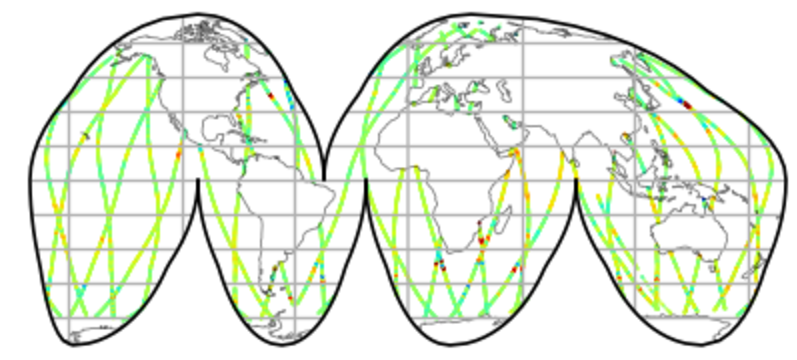
\includegraphics[width=\figwidthHalf]{figures/maps/altimeterCoverageEg.png}
  \caption{Illustration of spatial coverage of satellite altimeter; single day of Saral in May 2020. Observations near the coast are excluded from assimilation.}
  \label{fig:altimeterEg}
\end{figure}
%----------------------------------
SLA is a meaningful quantity to the extent that it is an anomaly from some reference, and that reference involves a spatial tide prediction; as introduced above in section \ref{sec:spatialTides}.
The role of tide predictions in mesoscale forecasts, and the handling of tides more generally, are taken up in the following sections.
%--------------------------------------------------
\subsection{Treatment of tides in nominally non-tidal \OGCM{}s}
\label{sec:tides_ogcm}
Operational \OGCM{}s in the \GODAE{} genealogy have intentionally focused on \emph{non-tidal} ocean dynamics. This focus has been motivated by the separation of time and length scales that allows for the simulation of relatively slow turbulent features at the mesoscale as a computationally tractable problem that can be adequately constrained by along-track altimeter observations.
In this view, much tidal variability is just the fast propagation of long wave length noise; a background sloshing of the barotropic ocean state not obviously connected to the evolution of eddies and boundary currents.
Moreover, the skill of spatial harmonic tide models in representing surface tides over the deep ocean facilitates the use of de-tided or filtered altimeter observations to constrain a mesoscale non-tidal simulation. In effect, the fluid simulation is split across two qualitatively distinct modelling approaches; an LTI frequency-space tidal ocean and a time-stepped turbulent mesoscale.  
\BL{} is a ``non-tidal'' system in that \ATGP{} forcing is not applied, and in contrast to local downscaled simulations, there are no lateral open boundary conditions. Not only does the mesoscale simulation exclude the gravitational tidal body forcing, it also excludes the surface boundary application of atmospheric pressure.   
Surface pressure is excluded as a forcing term for analogous time and length scale reasons as the tides.  And in fact for the barotropic mode the pressure and tidal forcing can be formulated in an identical manner as adjustments to the spatial gradient of the surface elevation as in \citet[Eq9.9.5]{gill1982atmosphere}.

The state variable quantifying surface elevation carried by the model is thus a peculiar sea level anomaly (SLA) that it a rather abstract  ....
which in itself is a rather abstract quantity. 
Using the \citet{Stevens:2001kb} nomenclature, \BL{} simulates an aggregated pseudofluid system with a qualified relationship to the actual ocean.



From that background, recent publications indicate a motivation towards more dynamic representation of the effects of ocean tides.   This is indicative of pervasive goal across numerical simulation practice to increase model concreteness by reducing the role of parameterisations \cite[section 5.3]{Petersen:2012tr}; a reduction of system aggregation \citep{Stevens:2001kb}.\\
Similarly, Griffies describes the ``general trend in ocean climate modelling towards reducing many of the common approximations'' \citep[pp20] {Griffies:2004vs}.
It could be said that the modelling community perceives parameterisations as a compromise that should ideally be replaced with explicit physics when computing power allows.  In spite of this, operational justification is a separate matter.

% split 
Timescales for depth-integrated barotropic and depth-dependant baroclinic ocean state are quite distinct and the design of \OGCM{}s have been influenced by this distinction. \\
%rigid ild
One approach has been to make the so-called `rigid-lid' approximation \cite[pp128]{gill1982atmosphere}. 
The rigid-lid by definition cannot represent explicit barotropic tides, and has other ramifications for ocean forecasting \cite[pp19]{Griffies:2004vs}.


% split explicit
A compromise strategy employed in \MOM{} (and other \OGCM{}s) is the so-called `split-explicit' scheme.    
In essence, cheap shallow-water barotropic dynamics are timestepped many times for each relatively expensive update of the full depth-dependant ocean state.  

Thus \MOM{} at face value is capable of representing barotropic surface tides.   However, there are several high level arguments against doing so.

One reason is the aims to which the model is being employed.  Much of the development of \OGCM{}s has been focused at climate times-scales, tipping the balance of away from the accuracy of high frequency sea level signals.   
Furthermore, in comparison to highly tuned tidal altases, simple and general barotropic can't be expected to achieve similar skill.


Filtered altimetry observations provide great value in observing and forecasting mesoscale eddies.
Treating tides as noise is reasonable insofar as the effects on the mesoscale structure are small relative to other source of error.


Decomposition of the dynamics into tractable categories for simulation is not aggregation per se, but it certainly does have implications for the role of parameterisations.  

From the perspective of \emph{users} of ocean forecasts there is basically no inherent value in decomposition.   
 
%-----------------%
\subsection{Motivation to explicitly simulate tidal effects}

Excluding tides from a mesoscale ocean simulation is essentially an undesirable but necessary design choice found to facilitate operational forecasting.
Barotropic tides interact with the baroclinic structure of the ocean, which in turn modulates the behaviour of barotropic waves; but the question as to if and to what extent these interactions can be paramaterised or ignored must be answered within practical constraints.
But design constraints are re-evaluated periodically; especially in light of the ongoing improvements in computational capacity and observation coverage.
Computational costs have reduced dramatically over the last decade and there is a motivation  to more explicitly simulate the role of tides in \OGCM{}s.
This motivation is primarily directed at representing the influence of barotropic tidal motions on the baroclinic mesoscale structure of the ocean state; not at directly improving the representation of total sea level.

Overall the tendency of geophysical simulation is towards every higher fidelity and concreteness - as discussed above. But the particular targets for a which some explicit simulation of tides in \OGCM{}s are aimed include:
\begin{itemize}
    \item improved spatial distribution of vertical mixing;
    \item improved simulation of barotropic/baroclinic energy conversion;
    \item improved resolution of frontal features;
\end{itemize}
These aims do not necessarily motivate an accurate simulation of the sea surface elevation.
Rather, in the spirit of Figure \ref{fig:ogcmScales}, it is a configuration with regard to what processes are relegated to sub-gridscale parameterisations.
Thus in the \OFAM{} simulations of \cite{Schiller:2004fv},  it was reasonable to include only a small subset of tidal constituents and effectively ignore realistic astronomical phase information.  In contrast to a standard tide prediction,  the aim in this case was ultimately to improve the broad spatial distribution in which tidal currents influence mixing and water mass formation.
\cite{Arbic:2004wz} highlighted the `inordinately large' magnitudes allocated to drag parameterisations in tide simulations and the important role for barotropic to baroclinic energy  energy conversion.  
Following great advances with the explicit simulation of tides using HYCOM,   \cite{10.1016/j.ocemod.2019.02.008} still rely on tidal parameterisations for subgrid conversion processes in the form of depth-dependant M2 wave drag term.
Further discussion of the details and progress towards explicit resolution of tides in \OCGM{}s is relegated to Appendix \ref{appendix:globalTides}
To date, the motivation to include tides in \BL{} remains far from the operational schedule.



TBC comments about separating skill of model appraaoches ....how this fits with seamless plans....



%-----------------%
\subsection{Representation of coastal boundaries}

Figure \ref{fig:map_masks} shows the \BL{} coastal discretisation.



Special role of coastally trapped signals in Australia  
....taken up in Chapter \ref{chp:waveguide}




